% unused snippets

% Table showing the e-folding time scales for Hintereisferner, time scales as rows
% --------------------------------------------------------------------------------

\begin{table}[htp]
  \centering
  \ra{1.4}
  \caption{e-folding time scales for Hintereisferner (RGI60-11.00897) in response to a step change in climate of $\Delta T = $\SI{\pm0.5}{\celsius} relative to the average climate between 1912 and 1942. Time scales are computed for changes in ice volume, surface area and glacier length, denoted as $\tau_V$, $\tau_A$ and $\tau_L$, respectively. \textit{V/A scaling} refers to the \vas{} model, while \textit{Flowline} refers to the Open Global Glacier Model (OGGM).}
  \label{tab:hintereisferner_time_scales}
  \begin{tabular}{@{}llccccc@{}}
    \toprule
    {} & \phantom{.} & \multicolumn{2}{c}{\textbf{V/A scaling}} & \phantom{ab} & \multicolumn{2}{c}{\textbf{Flowline}} \\
    \cmidrule{3-4}\cmidrule{6-7}
    \textbf{Time scales} & & \SI{-0.5}{\celsius} & \SI{+0.5}{\celsius} & & \SI{-0.5}{\celsius} & \SI{+0.5}{\celsius} \\
    \midrule
    $\bm{\tau_V}$ \textbf{[\si{\year}]} & & 39 & 36 & & 139 & 79 \\
    $\bm{\tau_A}$ \textbf{[\si{\year}]} & & 57 & 52 & & 159 & 107 \\
    $\bm{\tau_L}$ \textbf{[\si{\year}]} & & 85 & 80 & & 174 & 123 \\
    \bottomrule
  \end{tabular}
\end{table}

% Table showing the Hintereisferner equilibrium values, geometries as rows, no intital values
% -------------------------------------------------------------------------------------------

\begin{table}[htp]
  \centering
  \ra{1.4}
  \caption{Hintereisferner (RGI60-11.00897) equilibrium values after 1000 years of model evolution under a constant equilibrium climate with a temperature bias of \SI{-0.5}{\celsius} and \SI{+0.5}{\celsius}, respectively. Percentage values in parenthesis indicate normalized values in respective to their initial values.}
  \label{tab:hintereisferner_equilibrium_values}
  \begin{tabular}{@{}lrlcrlcrlcrl@{}}
    \toprule
    {} & \multicolumn{5}{c}{$\bm{\Delta T}$\textbf{ = \SI{-0.5}{\celsius}}} & \phantom{a} & \multicolumn{5}{c}{$\bm{\Delta T}$\textbf{ = \SI{+0.5}{\celsius}}} \\
    \cmidrule{2-6} \cmidrule{8-12}

    {} & \multicolumn{2}{c}{V/A scaling} & \phantom {} & \multicolumn{2}{c}{Flowline} & \phantom{a} & \multicolumn{2}{c}{V/A scaling} & \phantom {} & \multicolumn{2}{c}{Flowline} \\
    \midrule
    \textbf{Volume [\si{\cubic\kilo\meter}]} &  0.70 & (117\%) & \phantom {} &  1.37 & (171\%) & \phantom{a} &  0.50 & (84\%) & \phantom {} &  0.47 & (58\%) \\
    \textbf{Area [\si{\square\kilo\meter}]} &  9.02 & (112\%) & \phantom {} &  10.68 & (133\%) & \phantom{a} &  7.08 & (88\%) & \phantom {} &  6.17 & (77\%) \\
    \textbf{Length [\si{\kilo\meter}]} &  5.26 & (107\%) & \phantom {} &  9.95 & (144\%) & \phantom{a} &  4.52 & (92\%) & \phantom {} &  4.20 & (61\%) \\
    \bottomrule
  \end{tabular}
\end{table}

% Table showing the Hintereisferner equilibrium values, geometries as rows, vertical version
% ------------------------------------------------------------------------------------------

\begin{sidewaystable}[htp]
  \centering
  \ra{1.4}
  \caption{Hintereisferner (RGI60-11.00897) equilibrium values after 1000 years of model evolution under a constant equilibrium climate with a temperature bias of \SI{-0.5}{\celsius} and \SI{+0.5}{\celsius}, respectively. Percentage values in parenthesis indicate normalized values in respective to their initial values.}
  \label{tab:hintereisferner_equilibrium_values}
  \begin{tabular}{@{}lcccrlcrlcrlcrl@{}}
    \toprule
    % first level header
    {} & \multicolumn{2}{c}{\textbf{Initial values}} & \phantom{asdf} & \multicolumn{5}{c}{$\bm{\Delta T}$\textbf{ = \SI{-0.5}{\celsius}}} & \phantom{a} & \multicolumn{5}{c}{$\bm{\Delta T}$\textbf{ = \SI{+0.5}{\celsius}}} \\
    % second level header
    \cmidrule{2-3} \cmidrule{5-9} \cmidrule{11-15}
    {} & V/A scaling & Flowline & \phantom {} & \multicolumn{2}{c}{V/A scaling} & \phantom {} & \multicolumn{2}{c}{Flowline} & \phantom{a} & \multicolumn{2}{c}{V/A scaling} & \phantom {} & \multicolumn{2}{c}{Flowline} \\
    % table body
    % volume
    \midrule
    \textbf{Volume [\si{\cubic\kilo\meter}]} & 0.60 & 0.80 & &  0.70 & (117\%) & \phantom {} &  1.37 & (171\%) & \phantom{a} &  0.50 & (84\%) & \phantom {} &  0.47 & (58\%) \\
    % area
    \textbf{Area [\si{\square\kilo\meter}]} & 8.04 & 8.04 & &  9.02 & (112\%) & \phantom {} &  10.68 & (133\%) & \phantom{a} &  7.08 & (88\%) & \phantom {} &  6.17 & (77\%) \\
    % length
    \textbf{Length [\si{\kilo\meter}]} & 4.89 & 6.90 & & 5.26 & (107\%) & \phantom {} &  9.95 & (144\%) & \phantom{a} &  4.52 & (92\%) & \phantom {} &  4.20 & (61\%) \\
    \bottomrule
  \end{tabular}
\end{sidewaystable}

Text with all the equilibrium values contained in the table, don't know if to inlcude since it looks/reads weird.
The equilibrium ice volume for the positive and negative mass balance scenario is \SI{0.70}{\cubic\kilo\meter} (\SI{117}{\percent}) and \SI{0.50}{\cubic\kilo\meter} (\SI{84}{\percent}) for the \vas{} model and \SI{1.37}{\cubic\kilo\meter} (\SI{171}{\percent}) and \SI{0.47}{\cubic\kilo\meter} (\SI{58}{\percent}) for the flowline model, respectively. The values in parenthesis are normalized with the respective initial values. The equilibrium surface area for the positive and negative mass balance scenario is \SI{9.02}{\squared\kilo\meter} (\SI{112}{\percent}) and \SI{7.08}{\squared\kilo\meter} (\SI{88}{\percent}) for the \vas{} model and \SI{10.68}{\squared\kilo\meter} (\SI{133}{\percent}) and \SI{6.17}{\squared\kilo\meter} (\SI{77}{\percent}) for the flowline model, respectively. The equilibrium length for the positive and negative mass balance scenario is \SI{5.26}{\kilo\meter} (\SI{107}{\percent}) and \SI{4.52}{\kilo\meter} (\SI{92}{\percent}) for the \vas{} model and \SI{9.95}{\kilo\meter} (\SI{144}{\percent}) and \SI{4.20}{\kilo\meter} (\SI{61}{\percent}) for the flowline model, respectively.

% Time series for the HISTALP commitment run...

\begin{figure}[htp]
  \centering
  \begin{subfigure}[b]{0.99\textwidth}
    \caption{Normalized glacier volume}
    \label{fig:histalp_commitment:volume_norm}
    \centering
    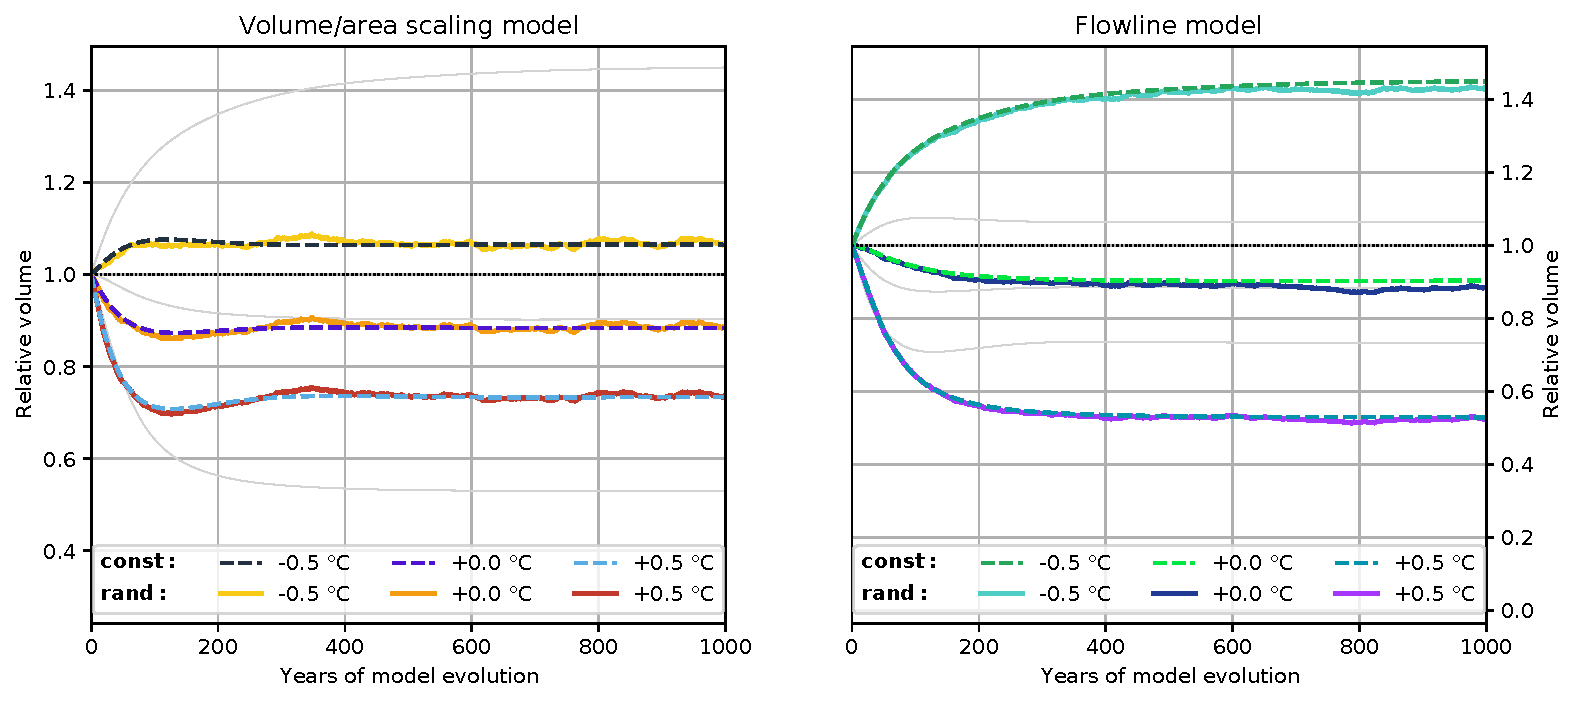
\includegraphics[width=\textwidth]{../plots/final_plots/time_series/histalp_commitment/volume_norm.pdf}
  \end{subfigure}
  \begin{subfigure}[b]{0.99\textwidth}
    \caption{Absolute glacier volume}
    \label{fig:histalp_commitment:volume_abs}
    \centering
    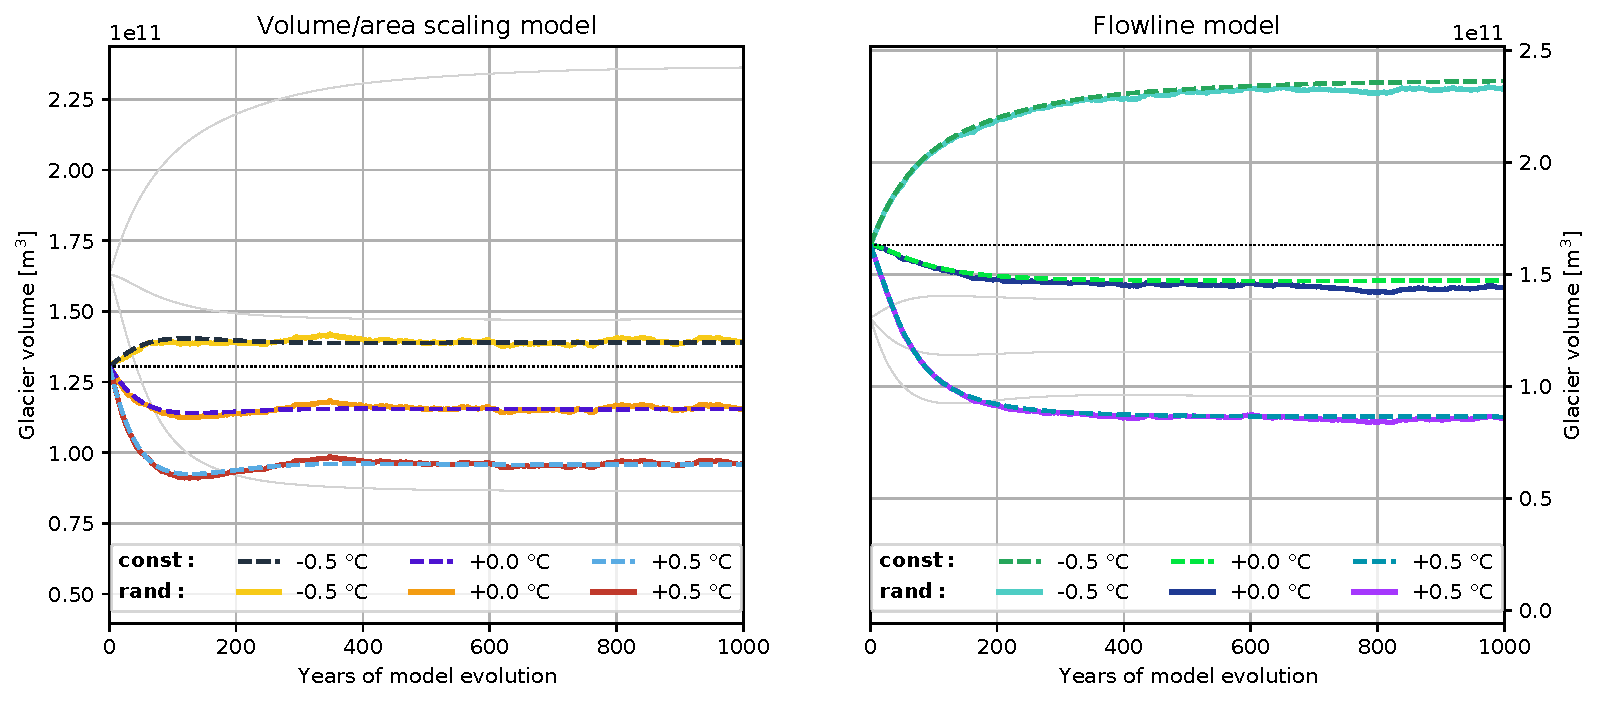
\includegraphics[width=\textwidth]{../plots/final_plots/time_series/histalp_commitment/volume_abs.pdf}
  \end{subfigure}
  
  \caption{Time series of total ice volume for all glaciers in the HISTALP domain. The upper two panels show the relative values, normalized with the initial values, while the lower two panels show absolute values. The left panels show the result of the \vas{} model, the right panels show the results of the flowline model. Solid lines represent a random climate scenario, while dashed lines represent a constant climate scenario. All climate scenarios are based on an equilibrium climate, however with three different temperature biases.
  Yellow, orange and red solid lines represent the \vas{} model, while cyan, blue and purple solid lines represent the flowline model, under a random climate with a temperature bias of \SI{-.5}{\celsius}, \SI{0}{\celsius} and \SI{+.5}{\celsius}, respectively. Yellow, orange and red dashed lines represent the \vas{} model, while cyan, blue and purple dashed lines represent the flowline model, under a constant climate with a temperature bias of \SI{-.5}{\celsius}, \SI{0}{\celsius} and \SI{+.5}{\celsius}, respectively. %TODO change colors
  The dotted line indicate the initial volume. The light gray lines represent the volume evolutions of the other model, to facilitate comparisons.}
  \label{fig:histalp_commitment}
\end{figure}